\documentclass[12pt]{article}
\usepackage[utf8]{inputenc}
\usepackage{amssymb,amsmath,amsfonts,eurosym,geometry,ulem,caption,color,xcolor,multicol,setspace,sectsty,comment,footmisc,caption,natbib,pdflscape,subfigure,array,hyperref,verbatim,mathpazo,longtable,ntheorem,siunitx,booktabs,threeparttable,afterpage}
%\usepackage[normalem]{ulem}
\usepackage[pdftex]{graphicx}
\graphicspath{{Imagens/}}
\usepackage{fullpage}
\usepackage{indentfirst}
\usepackage{changepage}

%\setlength{\pdfpagewidth}{8.5in} \setlength{\pdfpageheight}{11in}
%\setlength{\textheight}{8.5in} \setlength{\topmargin}{0.0in}
%\setlength{\headheight}{0.0in} \setlength{\headsep}{0.0in}
%\setlength{\leftmargin}{0.5in}
%\setlength{\oddsidemargin}{0.0in}
%\setlength{\parindent}{2em}
%\setlength{\parskip}{\baselineskip}%
%\setlength{\textwidth}{6.5in}
%\linespread{1.6}

\newcommand{\sym}[1]{\rlap{#1}}% Thanks to David Carlisle

\newcommand*{\captionsource}[2]{%
  \caption[{#1}]{%
    #1%
    \\\hspace{\linewidth}%
    \textbf{Source:} #2%
  }%
}
\newcommand{\horrule}[1]{\rule{\linewidth}{#1}} % Create horizontal rule command with 1 argument of height

%***************************************************
% Fix input with \midrule problem
%***************************************************

\makeatletter
\newcommand\primitiveinput[1]
{\@@input #1 }
\makeatother


\onehalfspacing
\newtheorem{theorem}{Theorem}
\newtheorem{corollary}[theorem]{Corollary}
\newtheorem{proposition}{Proposition}
\newenvironment{proof}[1][Proof]{\noindent\textbf{#1.} }{\ \rule{0.5em}{0.5em}}

\newtheorem{hyp}{Hypothesis}
\newtheorem{subhyp}{Hypothesis}[hyp]
\renewcommand{\thesubhyp}{\thehyp\alph{subhyp}}

\newcommand{\red}[1]{{\color{red} #1}}
\newcommand{\blue}[1]{{\color{blue} #1}}

\newcolumntype{L}[1]{>{\raggedright\let\newline\\arraybackslash\hspace{0pt}}m{#1}}
\newcolumntype{C}[1]{>{\centering\let\newline\\arraybackslash\hspace{0pt}}m{#1}}
\newcolumntype{R}[1]{>{\raggedleft\let\newline\\arraybackslash\hspace{0pt}}m{#1}}

\geometry{left=1.2in,right=1.2in,top=1.2in,bottom=1.2in}
\begin{document}
	
	\begin{titlepage}
		\title{The Impact of Bank Regulation on  Firms' Capital Structure: Evidence from Multinationals}
		
		\author{Lucas Avezum \and Harry Huizinga \and Louis Raes\thanks{Lucas Avezum: CentER, Tilburg University.Email:
				l.avezum@uvt.nl (corresponding author). Harry Huizinga: CentER, Tilburg University, CEPR. Louis Raes: CentER and EBC, Tilburg University.}}
		\date{\today}
		\maketitle
		\begin{abstract}
			\noindent This paper studies how bank regulatory policies relate to non-financial firms' capital structure. We first present a model where regulation affects banks' break even condition which in turn are transmitted to firms' leverage through their cost of debt. We empirically identify this effect by comparing firms within multinational corporations hosted in countries with differences in bank regulation. Our results show that tighter capital stringency and greater official supervisory power are negatively associated with firms' financial leverage while restriction on banking activities, ownership of non-financial firms and better external governance have the opposite effect.  \\
			\vspace{0in}\\
			\noindent\textbf{Keywords:} capital structure, bank regulation, multinational corporation\\
			\vspace{0in}\\
			\noindent\textbf{JEL Codes:} G28, G32, F23 \\
			
			\bigskip
		\end{abstract}
		\setcounter{page}{0}
		\thispagestyle{empty}
	\end{titlepage}
	\pagebreak \newpage
	
	
	\normalem
	
	\doublespacing
	
	
	\section{Introduction} \label{sec:introduction}
	As \cite*{blinder2017necessity} documented, the mandate of central banks has expanded considerably. Triggered mostly by the 2008 financial crisis, financial stability is now perceived by many central banks as a goal together with price stability. To achieve the former, several macroprudential instruments were included or extended in the toolboxes of central bankers and other supervisory authorities, reshaping the bank regulatory framework across the globe. \cite*{barth2013bank} show that several measures for bank regulation and supervision have changed significantly between 1999 and 2011. Although the effects on the bank sector of regulatory policies have been extensively studied (\cite*{barth2013}; \cite*{anginer2014does}; \cite*{caprio2014macro};\cite*{demirguc2013bank}), there is little evidence of their impact on non-financial sectors of the economy. 
	
	In this paper we study how bank regulation and supervision relate to non-financial firms' capital structure. We focus on multinational firms for our empirical identification strategy. We first present a model of the multinational corporation's optimal capital structure, based on \cite*{huizinga2008capital}. This model considers the trade-off between tax advantages of debt versus the bankruptcy and agency costs related to it. We add to this model the transmission of bank regulatory policies to firms' cost of debt. Our theoretical model provides predictions on the impact of regulatory policies on firms' financial leverage. Regulation affects banks' funding and operational costs which may be translated in changing lending conditions. We expect multinationals' capital structure to reflect differences among regulation and supervision in the countries where they are hosted. Hence, multinational groups could potentially be a transmission channel of bank regulation international spillover, as the latter creates incentive for multinationals to shift debt across their subsidiaries. 
	
	Empirical evidence on the impact of bank regulatory policies on firms' capital structure is provided for a sample of 64,490 firms hosted in 24 countries and belonging to 9,913 multinational corporate groups from the Bureau van Dijk Orbis dataset. Our identification strategy relies on two aspects of the data: first, firm-level data mitigate endogeneity concerns as the leverage level of a single non-financial firm is not likely to be considered by supervision authorities when deciding on bank regulation; and second, with ownership information we can track multinational groups and exploit the variation in bank regulatory policies across firms of each group within the same period. On the basis of demand factors alone, the optimal leverage level does not have to be constant in time. Consequently, multinational or firm fixed effects do not account for all the time varying unobservable characteristics of firms. The inclusion of year fixed effects is not sufficient since it does not capture cross-firm unobservable variability in demand. Thus, our dataset allows us to include multinational$\times$year fixed effects, effectively controlling for those unobservable characteristics. We also add industry fixed effects to ensure that our conclusions are not the result of sector specific factors on optimal leverage. 
	
	Overall, the results show that on average one standard deviation tighter capital stringency and greater official supervisory power relate to firms' financial leverage being 1.2 p.p. and
	0.5 p.p. lower, respectively, while one standard deviation higher restrictiveness on banking activities, financial conglomerates and better external governance are associated with 1.3 p.p., 1.0 p.p., and 1.8 p.p. higher financial leverage, respectively. Although the effects are small relative to the sample standard deviation of leverage (27 p.p.), they are not negligible, specially if considered together and in comparison to the effect of other variables considered as important determinants of firms' capital structure (for instance, one standard deviation of profitability and size are associated with leverage being 3.0 p.p. lower and 3.6 p.p. higher, respectively). Moreover, we find no evidence of multinational corporations taking advantage of differences in bank regulation as our theoretical model predicts. Still, the capital structure of multinational firms reflects differences in corporate taxes, corroborating to our assumption that leverage decisions for each subsidiary is taken at the multinational level. 
	
	Research on the effects of bank regulation, such as, prudential policies has increased considerably after the 2008 financial crisis. Several authors rely on cross-country aggregate data to study the relationship between macroprudential policies and financial indicators. \cite*{cerutti2015use} introduces a dataset containing the usage of 12 macroprudential policies at 119 countries from 2000 to 2013. They document that prudential instruments are mostly used in developing countries where they also appear to be more effective. Among their findings, borrower-related policies, such as limits on loan-to-value and debt-to-income ratios are associated with reductions in credit growth and house prices. The author also provide an extensive review of the literature on macroprudential policies. As mentioned, most of the literature focus on the effects of regulation and supervision on the bank and financial sectors. Two recent exceptions are \cite*{ayyagari2017credit} who use firm-level data to relate macroprudential policies across 119 countries to firms' debt growth and \cite*{epure2017household} who studies with loan-level data the impact of macroprudential tools on household credit in Romania.    
	
	Finally, this paper also builds on the capital structure literature. Many papers study the determinants of firms' leverage, both theoretical and empirically. \cite*{titman1988determinants} and more recently, \cite*{oztekin2015capital} provide an overview of and test the different proposed capital structure's determinants. Following the literature's findings, we control for several firm characteristics such as, profitability, tangibility, growth opportunities, firm size and riskiness. Besides highlighting bank regulation as another determinant of capital structure, to our knowledge, we are the first to use variation across firms belonging to a multinational group as an identification strategy to isolate supply from demand factors.          
	
	The paper proceeds as follows: section \ref{sec:model} presents the model and section \ref{sec:data} describes the data. The empirical strategy is described in section \ref{sec:strategy} while the results are discussed in section \ref{sec:result}. Section \ref{sec:robustness} presents some robustness tests and extensions and section \ref{sec:conclusion} concludes. 
	
		\section{Model} \label{sec:model}
	In this section we present a model of the optimal capital structure of multinationals based on \cite{huizinga2008capital} who consider tax and non-tax factors in the firms' decision problem. We extend their model by allowing bank regulatory tools to affect the cost of debt to firms and consequently their optimal leverage level.  
	\subsection{Bank regulation and cost of debt}
	\label{subsec:bank}
	We assume risk neutral banks operating in a competitive market, hence, banks choose the interest rate charged ($r$) to their borrowers in order to break even in expectation. We consider the problem of a bank perpetually financing a project by $P$ either with debt $L$ or equity $E$, that is, $P=E+L$. The bank does not have full information of the project and, therefore, estimates the perpetual return of the project $R$ to follow a uniform distribution on the interval $[\underline{R},\overline{R}]$ with $\underline{R}\leq0$ and $\underline{R}>0$. We call $\sigma^2=(\underline{R}-\overline{R})^2/12$ the sensitivity to the project's risk by the bank. On the liability side, the bank has two options of funding: deposits $D$ and capital $C$, that is, $P=D+C$. Deposits charge the discount rate of the economy $\delta$ while there is a premium to capital $\delta+\epsilon$. Moreover, the bank has an outside option with value $K$.
	
	The bank sector is regulated. First, the outside option is restricted, meaning a lower value of $K$. Second, the amount of equity that the bank can hold is limited to $\alpha P$. Third, capital requirements are imposed, meaning $K(L+E)\ge\kappa$. In optimum, this condition will always hold in equality. Fourth, stronger official supervisory power means banks are less likely to engage in risky projects. In our model this policy is translated in higher estimated risk for the project $\sigma$. Finally, better external governance reduces adverse selection, by improving and extending the set of information that banks must provide. If we call the governance level $g$, in our model, an increase in $g$ results in a lower capital premium, that is, $\epsilon'(g)<0$.
	
	Taking all the information above, the break even condition for a bank can be written as:  
	
		\begin{equation}
	\begin{aligned}
	Q=\alpha\int_{rL}^{\overline{R}}\frac{(R-rL)(1-\tau)}{\underline{R}-\overline{R}}dR+\int_{rL}^{\overline{R}}\frac{rL}{\underline{R}-\overline{R}}dR+\int_{\underline{R}}^{rL}\frac{R}{\underline{R}-\overline{R}}dR-\delta D-(\delta+\epsilon)K
	\end{aligned}
	\label{eq:break even}
	\end{equation}
	
	Competitive market means that the financing activity must equate to the outside option $Q$. The first term on the right hand side is the share of the firm's expected value that the bank hold via equity. Note, that this term takes into account the tax ($\tau$) benefit of debt. The second and third terms are the expected value from debt. The fourth and fifth are the cost of funding via deposit and capital, respectively. Solving the integrals and using the capital requirement, ownership condition, the definition of sensitivity to risk, the bank's balance sheet $P=D+K=L+E$ and the fact that the capital premium is a function of $g$ we rewrite equation \ref{eq:break even}:
		
			\begin{equation}
		\begin{aligned}
		Q=\frac{(1-\alpha)P\overline{R}r}{\sigma2\sqrt{3}}[1-\alpha(1-\tau)]+\frac{\alpha(1-\tau)\overline{R}^2}{\sigma2\sqrt{3}}-\frac{\underline{R}^2}{\sigma2\sqrt{3}}-\delta P-\epsilon(g)P\sigma\kappa,
		\end{aligned}
			\label{eq:break even solved}
		\end{equation} 
	and rearranging terms:
		\begin{equation}
	\begin{aligned}
	r=&\frac{Q\sigma2\sqrt{3}}{(1-\alpha)P\overline{R}(1-\alpha(1-\tau))}-\frac{\alpha(1-\tau)\overline{R}}{(1-\alpha)(1-\alpha(1-\tau))P}\\
	&+\frac{\underline{R}^2}{(1-\alpha)P\overline{R}(1-\alpha(1-\tau))}+\frac{(\delta+\epsilon(g)\sigma\kappa)\sigma2\sqrt{3}}{(1-\alpha)\overline{R}(1-\alpha(1-\tau))}.	\end{aligned}
		\label{eq:interest rate}
	\end{equation} 
	
	From equation \ref{eq:interest rate} we can find the effect of each regulatory change on interest rate: 
		\begin{equation}
	\frac{\partial r}{\partial Q}>0, \ \frac{\partial r}{\partial \alpha}>0, \
	\frac{\partial r}{\partial \kappa}>0, \
	\frac{\partial r}{\partial \sigma}>0, \
	\frac{\partial r}{\partial g}<0,
		\label{eq:derivatives}
	\end{equation}
	with the condition that $\alpha<\frac{(2-\tau)}{2(1-\tau)}-\frac{\overline{R}}{2Pr}$ for the derivative with respect to $\alpha$. Hence, the bank's equity share has to be small enough. Otherwise, it will be beneficial to the bank to compensate lower share in the firm's equity by increasing the value of the firm by charging lower interest rate. 
	       
	\subsection{Balance sheets and financial leverage}
	\label{subsec:balancesheet}
	We consider a multinational group that is composed of $n-1$ subsidiaries and the parent firm. Each subsidiary has assets $A_i$ and is financed by external debt $L_i$ and the parent firm's equity $I_i$. For a subsidiary $i$ the balance sheet is:
	\begin{equation}
	\begin{aligned}
	A_i=I_i+L_i, \quad i=1,...,n.
	\end{aligned}
	\label{eq:sub balance sheet}
	\end{equation}
	
	We assume that the parent firm is the sole owner of each subsidiary. Hence, if $A_p$, $E_p$ and $L_p$ are, respectively, the assets, equity and debt of the parent firm, its balance sheet can be stated as: 
	\begin{equation}
	\begin{aligned}
	A_p+\sum_{i=1}^{n-1}I_i=E_p+L_p. 
	\end{aligned}
	\label{eq:parent balance sheet}
	\end{equation}
	
	Financial leverage ($\lambda_i$) is defined as total non-equity liabilities to total assets, that is, $\lambda_i=L_i/A_i$. Replacing equation \ref{eq:sub balance sheet} in equation \ref{eq:parent balance sheet}, at the multinational level, total leverage becomes:
	\begin{equation}
	\begin{aligned}
	\lambda_m=\frac{\sum_{i=1}^{n}L_i}{\sum_{i=1}^{n}A_i}=\sum_{i=1}^{n}\lambda_i\rho_i, 
	\end{aligned}
	\label{eq:total leverage}
	\end{equation} 
	where $\rho_i=A_i/\sum_{i=1}^{n}A_i$ is the asset share of firm $i$ within the multinational. The second equality in equation \ref{eq:total leverage} is reached by replacing the definition of leverage for a subsidiary in the first equality of the same equation. Equation \ref{eq:total leverage} shows that leverage at the multinational level can be seen as the weighted average of the subsidiaries and parent firms' financial leverage by their respective asset share. Adjustments in the capital structure are assumed to be the result of changes in liabilities rather than assets, that is, assets are taken as given to firms. 
	
	\subsection{Costs associated with leverage}
	\label{subsec:costs}
	We assume that the debt of any subsidiary firm is implicitly or explicitly guaranteed by the parent firm. Consequently, the expected cost of bankruptcy associated with higher leverage is contemplated at the multinational level. A quadratic expected bankruptcy cost function ($C_m$) is considered as follows:
	
	\begin{equation}
	\begin{aligned}
	C_m=\frac{\gamma}{2}\lambda_m^2\bigg(\sum_{i=1}^{n}A_i\bigg).
	\end{aligned}
	\label{eq:cost bankruptcy}
	\end{equation}
	
	We also consider costs at the subsidiary level which are related to incentives that leverage brings to local managers. As an example, high leverage, on the one hand, may inhibit overspending. On the other hand it can lead to unnecessarily risk-averse managers. Let $\lambda^*$ be the optimal leverage ratio when considering only the incentives to local managers. The cost of deviating from $\lambda^*$ is assumed to be quadratic and proportional to the amount of asset at establishment $i$ as follows:  
	
	\begin{equation}
	\begin{aligned}
	C_i=\frac{\mu}{2}(\lambda_i-\lambda^*)^2A_i-\frac{\mu}{2}(\lambda^*)^2A_i, \quad i=1,...,n.
	\end{aligned}
	\label{eq:agency cost}
	\end{equation}
	
	Lastly, we include the cost of debt derived in section \ref{subsec:bank}. For tractability we summarize equation \ref{eq:interest rate} as the following:
	\begin{equation}
	\begin{aligned}
	r_i=\delta_i(1+\phi'\Pi_i), \quad i=1,...,n.
	\end{aligned}
	\label{eq:cost of debt}
	\end{equation}
	where $\phi$ is a parameter vector containing the derivatives specific to the set of regulatory and supervision instruments $\Pi$ implemented in the country of firm $i$.	
	
	\subsection{Multinational's value}
	\label{subsec:value}
	Let $R_i$ be the gross revenue of firm $i$, which is assumed to be positive and constant. The value of firm $i$, if fully financed by equity, is the discounted cash flow considering perpetuity minus the corporate tax payments 
	\begin{equation}
	\begin{aligned}
	V_i^U=\frac{R_i}{\delta_i}(1-\tau_{i}), \quad i=1,...,n,
	\end{aligned}
	\label{eq:v_u}
	\end{equation}	
	where $\tau_{i}$ is the effective corporate tax rate charged to firm $i$. The discount and tax rates are expected by the firm to not vary. Next, we consider firm $i$'s value with external financing $L_i$ and the costs associated with leverage (equation \ref{eq:agency cost})
	\begin{equation}
	\begin{aligned}
	V_i^L=L_i+\frac{(R_i-r_iL_i)}{\delta_i}(1-\tau_{i})-C_i, \quad i=1,...,n,
	\end{aligned}
	\label{eq:v_l_1}
	\end{equation}	
	where the fact that interest rate payments are deductible from taxable income is accounted for. Replacing equations \ref{eq:cost of debt} and \ref{eq:v_u} on the value function \ref{eq:v_l_1} and rearranging terms we reach the following expression for the value of the firm:
	\begin{equation}
	\begin{aligned}
	V_i^L=V_i^U+\tau_{i}L_i-\phi'\Pi_iL_i+\tau_{i}\phi'\Pi_iL_i-C_i, \quad i=1,...,n.
	\end{aligned}
	\label{eq:v_l_2}
	\end{equation}	
	The second term of the right hand side is the debt tax shield. The third term is the effect of bank regulation through the cost of debt. Abstracting from taxes, higher interest payments decrease cash flow and consequently the value of the firm. The fourth term reflects the interaction between cost of debt and tax payments. Higher interest rates decrease taxable income and, considering this effect alone, increase after-tax cash flow.
	
	The value of the multinational corporation $m$ is equal to the sum of equation \ref{eq:v_l_2} for each subsidiary and parent firms minus the expected cost of bankruptcy (equation \ref{eq:cost bankruptcy}) as shown in the following equation:
	\begin{equation}
	\begin{aligned}
	V_m^L=V_m^U+\sum_{i=1}^{n}\tau_iL_i-\phi'\sum_{i=1}^{n}\Pi_iL_i+\phi'\sum_{i=1}^{n}\tau_i\Pi_i L_i-C_m-\sum_{i=1}^{n}C_i
	\end{aligned}
	\label{eq:v_l}
	\end{equation}
	where $V_m^L$, and $V_m^U$ are the multinational's values when leveraged and completely unleveraged, respectively.
	\subsection{Optimal leverage}
	\label{subsec:opt_leverage}
	The multinational corporation's objective is to maximize its value by choosing each establishment's (subsidiaries and parent firm) debt level taking into account the costs and benefits associated with leverage. The problem can be stated as follows:
	\begin{equation}
	\begin{aligned}
	\max_{L_i}V_m^U+\sum_{i=1}^{n}\tau_iL_i-\phi'\sum_{i=1}^{n}\Pi_iL_i+\phi'\sum_{i=1}^{n}\Pi_i\tau_i L_i-C_m-\sum_{i=1}^{n}C_i, \quad i=1,...,n.
	\end{aligned}
	\label{eq:problem}
	\end{equation}
	
	The first order conditions of the problem \ref{eq:problem} are:
	\begin{equation}
	\begin{aligned}
	\tau_i-\phi'\Pi_i+\phi'\Pi_i\tau_{i}-\gamma\lambda_m-\mu(\lambda_i-\lambda^*)=0, \quad i=1,...,n\\
	\end{aligned}
	\label{eq:FOC}
	\end{equation}
	which, together with equation \ref{eq:total leverage} can be written as:  
	\begin{equation}
	\mu\lambda_i=\mu\lambda^*+\tau_{i}-\phi'\Pi_i+\phi'\Pi_i\tau_{i}-\gamma \sum_{j=1}^{n}\lambda_j\rho_j, \quad i=1,...,n.
	\label{eq:FOC2}
	\end{equation}
	Subtracting the first order condition for a subsidiary $j$ from the first order condition for a subsidiary $i$ we find the following expression that relates the leverage ratios of firms $j$ and $i$ to the difference in tax rates, macroprudential tools and the interaction of them that the two firms are subjected to:
	\begin{equation}
	\begin{aligned}
	\lambda_j=\lambda_i-\frac{1}{\mu}(\tau_i-\tau_j)+\frac{\phi'}{\mu}(\Pi_i-\Pi_j)-\frac{\phi'}{\mu}(\Pi_i\tau_i-\Pi_j\tau_j).
	\end{aligned}
	\label{eq:joint FOC}
	\end{equation}
	Replacing equation \ref{eq:joint FOC} in \ref{eq:FOC2}, the optimal leverage level for subsidiary $i$ becomes:  
	\begin{equation}
	\begin{aligned}
	\lambda_i=&\theta_0\lambda^*+\theta_1\tau_i-\theta_2\Pi_i+\theta_3\sum_{j=1}^{n}(\tau_i-\tau_j)\rho_j-\theta_4\sum_{j=1}^{n}(\Pi_i-\Pi_j)\rho_j\\
	&+\theta_2\Pi_i\tau_{i}+\theta_4\sum_{j=1}^{n}(\Pi_i\tau_i-\Pi_j\tau_j)\rho_j, \quad i=1,...,n
	\end{aligned}
	\label{eq:optimal leverage in theory}
	\end{equation}
	where
	\begin{equation*}
	\begin{aligned}
	 \theta_0=\frac{\mu}{(\mu+\gamma)}, \ \theta_1=\frac{1}{(\mu+\gamma)}, \
	\theta_2=\frac{1}{(\mu+\gamma)}\phi', \
	\theta_3=\frac{\gamma}{\mu(\mu+\gamma)}, \
	\theta_4=\frac{\gamma}{\mu(\mu+\gamma)}\phi'.
	\end{aligned}
	\end{equation*}
	
    Equation \ref{eq:optimal leverage in theory} shows that the optimal leverage ratio at all establishments of the multinational depends on the incentives to local managers ($\lambda^*$) balanced by the cost of bankruptcy ($\theta_0$). The domestic effects of tax and bank regulatory policies are represented by $\theta_1\tau_i$, $\theta_2\Pi_i$ and their interaction $\theta_2\Pi_i\tau_i$. Lastly, the remaining terms reflect the extra incentive to shift debt that multinationals have, by taking advantage of differences in tax rate and bank regulation across host countries. In section \ref{sec:strategy} we build our empirical strategy based on equation \ref{eq:optimal leverage in theory}.
    
	\section{Data} \label{sec:data}	
	\subsection{Bank regulation} \label{subsec:MPI}
	
	We rely on the efforts of \cite*{barth2013bank} for our measures of bank regulation. This work introduces the fourth of a series of surveys conducted by the authors sponsored by the World Bank \footnote{Previous surveys are described and analyzed in \cite{barth2001regulation}, \cite{barth2004bank}, \cite{barth2008bank}}. Due to time restriction of our firm level dataset we can only use the last two surveys which provide information for 2011 and 2006 across 125 and 142 countries, respectively. The measures track bank regulatory and supervisory policies with summary indices that allow comparison across countries.

     We focus on five main indices. We add in parentheses the indices' numbers from the original dataset for reference:
      \begin{itemize}
     	\item \underline{Restriction on banking activities } (index I.IV): the extent to which banks may engage in securities, insurance and real estate activities (higher values indicate more restrictive). Restrictions on other activities mean lower outside option value, implying a positive sign of the estimated coefficient on leverage. Hence, the expected sign of the effect on leverage for this variable is positive.  
     	\item \underline{Financial conglomerates restrictiveness} (index II.IV): restrictions on banks' ownership of nonfinancial firms and on non-bank firms owning banks (higher values indicate more restrictive). Since equity investment on non-financial firms is restricted, banks have to rely more on debt instruments, suggesting a positive effect on leverage. 
     	\item  \underline{Capital regulatory strigency} (index IV.III): whether certain funds may be used to initially capitalize a bank and whether they are official and reflect risk elements (higher values indicate greater stringency). Higher capital stringency implies greater cost of capital and exposure for banks, consequently, we expect the estimated coefficient to be negative.
     	\item \underline{Official supervisory power} (index V.I): whether the supervisory authorities have the authority to take specific actions to prevent and correct problems (higher values indicate greater power). A greater power to intervene directly creates incentives to decrease risk-taking by banks, thus the effect on leverage should be negative.
     	\item \underline{External governance} (index X.V): tracks the quality and presence of certain accounting practices, financial statement transparency, external rating and auditing  (Higher values indicate better corporate governance). Better screening reduces adverse selection of banks in need of capital improving credit market conditions, which can be transmitted to banks' borrowers.
     \end{itemize} 
	  
	  We matched the information from the last survey to the firm level data for the years of 2011, 2010, 2009 and 2008. For 2007, we use the results from the previous survey (\cite{barth2008bank}).  
	   
	%  \begin{figure}[h!]
%	  	\centering
%	  	\caption{Box-plot of macroprudential policies indexes' data points}
%	  	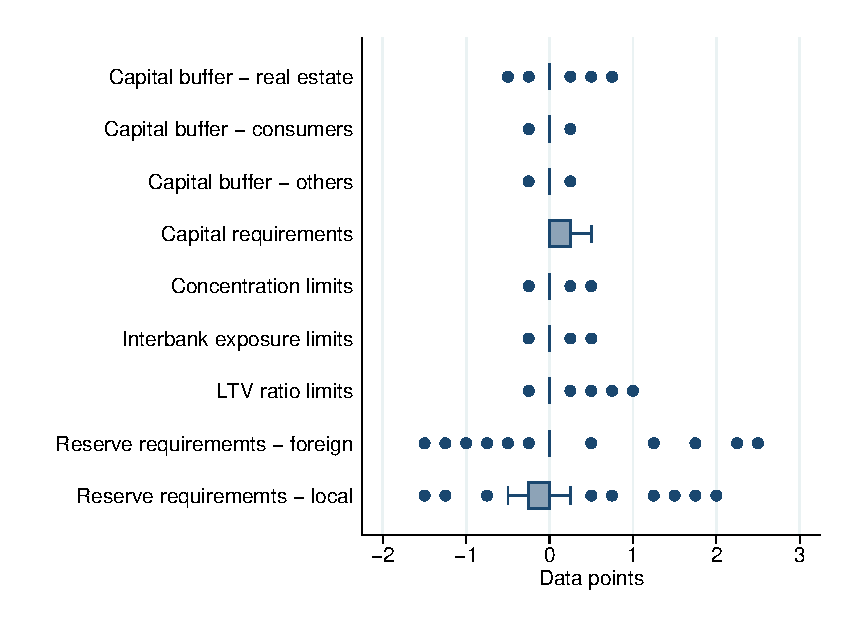
\includegraphics[scale=1.1]{C:/Users/User/work/master_thesis/analysis/output/graphs/box_plot_data.eps}
%	  	\label{fig:boxplot data}
%	  \end{figure} 
	  	
 	\subsection{Firm level} \label{subsec:firm}
	Firm level data and ownership relationships are taken from the Orbis database compiled by Bureau Van Dijk. The dataset consist of worldwide accounting and ownership information on both private and public owned companies. Ownership is considered if one firm owns at least 50\% of another firm's shares in a given year. We call the second a subsidiary firm. If a company owns one or more firms but is itself owned by another, this firm is called an intermediate and for all purposes is also considered as a subsidiary. A parent firm is the ultimate owner of a group, that is, a firm that owns one or more companies but none of its shareholders have more than 50\% of its shares.
	
	\begin{small}
		{\setstretch{1.0}
			\begin{longtable}{lrrrrrr}\\
				\label{tab:number of firms}\\
				\multicolumn{7}{c}{Table \ref{tab:number of firms} - Subsidiary firms' country distribution in benchmark panel}\\
				\hline \hline \addlinespace Country & 2007 & 2008 & 2009 & 2010 & 2011 & Total  \\
				\endfirsthead
				\multicolumn{7}{c}{Table \ref{tab:number of firms} - Subsidiary firms' country distribution of benchmark panel}\\
				\hline \hline \addlinespace Country & 2007 & 2008 & 2009 & 2010 & 2011 & Total  \\
				\hline \addlinespace \endhead
				\hline
				\multicolumn{7}{r}{{\textit{(Continued)}}}\\ \endfoot
				\\ 	
				\endlastfoot
				\primitiveinput{C:/Users/u1273941/Research/Projects/macroprudential_capital_structure/analysis/output/tables/summary/number_firms_table.tex}
				\hline 			
			\end{longtable}	
		}
	\end{small}
	
	Given our identification strategy, we keep only multinationals groups, that is, corporate groups that have firms in at least two countries.  Banks, insurance and financial related companies\footnote{We keep only firms with the Orbis type identifier "C".} and firms in the utility sector\footnote{Two digit NACE codes from 35 to 39.} are also excluded since their capital structure decisions are constrained by regulation. We also exclude firms with zero or negative asset and after constructing the leverage measures, we exclude observations where leverage is above one or below zero. Firms with negative net worth are likely to be credit constrained and therefore not able to choose their capital structure optimally. For our benchmark analysis, we balanced the panel across specifications, to be certain that our results are not driven by sample differences. We later relax this restriction as a robustness test.
	
		\begin{small}
		{\setstretch{1.0}
			\begin{longtable}{lrrrrrr}\\
				\label{tab:number of parent}\\
				\multicolumn{7}{c}{Table \ref{tab:number of parent} - Parent firms' country distribution in benchmark panel}\\
				\hline \hline \addlinespace Country & 2007 & 2008 & 2009 & 2010 & 2011 & Total  \\
				\endfirsthead
				\multicolumn{7}{c}{Table \ref{tab:number of parent} - Parent firms' country distribution of benchmark panel}\\
				\hline \hline \addlinespace Country & 2007 & 2008 & 2009 & 2010 & 2011 & Total  \\
				\hline \addlinespace \endhead
				\hline
				\multicolumn{7}{r}{{\textit{(Continued)}}}\\ \endfoot
				\\ 	
				\endlastfoot
				\primitiveinput{C:/Users/u1273941/Research/Projects/macroprudential_capital_structure/analysis/output/tables/summary/number_parent_table.tex}
				\hline 			
			\end{longtable}	
		}
	\end{small}

	The final sample consists of 69,490 firms from 2007 to 2011 resulting in 189,130 firm-year observations. Table \ref{tab:number of firms} provides information on the amount of firms per host country in our sample. We track firms in 24 countries, consequently, our analysis consists in comparing differences on bank regulation for those 24 countries. The dataset is highly concentrated in Europe: only 1,296 firm-year observations are from a country outside Europe. Also, note that we do not track the entire corporate group. Table \ref{tab:number of parent} shows the amount of parents per country and year in our sample. Several countries are included in \ref{tab:number of parent} but not in table \ref{tab:number of firms}, meaning that we do not observe those parent firms. Importantly, the distribution of parents is also highly concentrated in Europe, with 147,450 firm-year observations having parents within the tracked 17 European countries and 15,508 with parents from another country in Europe.
	
	Information about the size and composition of multinationals in the benchmark sample can be seen in table \ref{tab:info}. We track 9,913 multinationals in the sample period, or 25,509 multinational-year observations. Parent indicates if a firm-year observation is a parent. Around 37\% of all the observations are parent firms. The median amount of firms in a multinational in a given year is 4. However there are mega conglomerates of up to 874 firms. The median multinational is present in only 2 countries and owns firms in 2 sectors. The largest multinational, with respect to country coverage, is present in 12 countries while 56 is the number of sectors of the multinational with the widest range of activities.
	   
		\begin{small}
		{\setstretch{1.0}
			\begin{longtable}{lrrrrr}\\
				\label{tab:info}\\
				\multicolumn{6}{c}{Table \ref{tab:info} - Information on multinationals}\\
				\hline \hline \addlinespace  & Mean & SD & Min & Med & Max  \\
				\endfirsthead
				\multicolumn{6}{c}{Table \ref{tab:info} - Information on multinationals}\\
				\hline \hline \addlinespace    & Mean & SD & Min & Med & Max  \\ \hline  \endhead
				\hline
				\multicolumn{6}{r}{{\textit{(Continued)}}}\\ \endfoot
				\addlinespace
				\multicolumn{6}{p{9cm}}{{Notes: The sample period is 2007-2011. In our benchmark sample there are 9,913 multinational, resulting in 25,509 multinational-year observations. Parent is a dummy variable assigning 1 to final parent firms and 0 to subsidiaries}}\\  	
				\endlastfoot
				\primitiveinput{C:/Users/u1273941/Research/Projects/macroprudential_capital_structure/analysis/output/tables/summary/summary_mult.tex}
				\hline 			
			\end{longtable}	
		}
	\end{small}

	Statistics on firm level data are summarized in table \ref{tab:summary}. Financial leverage is defined as the ratio of total non-equity liabilities to total assets. All the spillover measures are constructed as described in section \ref{sec:strategy}. Among the control variables tangibility is the ratio of fixed assets to total assets. While tangible assets can be used as collateral, implying a positive relationship between tangibility and leverage, the depreciation of fixed assets reduces taxable income. Hence, tangible assets can also be substitute to debt as tax shield. We use the logarithm of fixed assets to proxy for firm size, which is expected to be positively associated to leverage. Profitability is the ratio of earning before interest, tax, depreciation and amortization (EBITDA) to total assets. Higher profits may facilitate access to credit but firms with larger cash flow may also opt to finance themselves with retained earnings as predicted by the pecking order theory of capital structure. Thus, the relationship between profitability and leverage is ambiguous. Opportunity is the median annual growth rate of sales in an industry in a particular country. We expect this variable to be positive associated to leverage as higher growth opportunities signal future profits that can be used to increase the ability to borrow in the present. Risk is the standard deviation of firms' profitability over the sample period and it is our proxy for the riskiness of firms. Finally, we winsorized all firm-level controls at the 1st and 99th percentile to remove the effect of outliers.
	
		\begin{small}
		{\setstretch{1.0}
			\begin{longtable}{lrrrrr}\\
				\label{tab:summary}\\
				\multicolumn{6}{c}{Table \ref{tab:summary} - Summary statistics of benchmark panel}\\
				\hline \hline \addlinespace  & Mean & SD & Min & Med & Max  \\
				\endfirsthead
				\multicolumn{6}{c}{Table \ref{tab:summary} - Summary statistics of benchmark panel}\\
				\hline \hline \addlinespace    & Mean & SD & Min & Med & Max  \\ \hline  \endhead
				\hline
				\multicolumn{6}{r}{{\textit{(Continued)}}}\\ \endfoot
				\addlinespace
				\multicolumn{6}{p{15cm}}{{Notes: The sample period is 2007-2011. The number of observations is 189,130.
						Financial leverage is trimmed at a maximum value of 1 and a minimum of 0. Firm variables are winsorized at the 1\% to minimize the impact of outliers. See Table \ref{tab:definition} for variable definitions
						and sources.}}\\ 	
				\endlastfoot
				\primitiveinput{C:/Users/u1273941/Research/Projects/macroprudential_capital_structure/analysis/output/tables/summary/summary.tex}
				\hline 			
			\end{longtable}	
		}
	\end{small}
 
\subsection{Country level} 
 \label{subsec:country}
	Table \ref{tab:number of firms} provides statistics at the country level. We control for political risk, exchange rate risk and law and order using the indices from the \textit{International Country Risk Guide}. We inverted the original risk indices, resulting in higher scores for greater risk. \cite*{kesternich2010afraid} find that political risk can both increase or decrease firm leverage. A more unstable political environment may discourage banks to provide loans, but parent firms might want to reduce their value at risk by leveraging their subsidiaries' operations. \cite*{burgman1996empirical} studies determinants of capital structure that differ between domestic and multinational corporations, finding political and exchange rate risk to be positively associated with leverage. The index for law and order proxy for the institutional level, which \cite*{demirgucc1998law} show to affect firms debt growth. Higher scores mean greater juridical strength.
	
	 We include four macro controls from the \textit{World Development Indicators} database from the World bank. Private credit to GDP is the share of credit to the private sector to GDP and is a proxy to financial development. We expect financial development to affect leverage positively. Inflation is the annual log change in the consumer price index. As \cite{huizinga2008capital} point out, an inflationary environment may discourage firms to borrow as risk premiums increase. GDP growth rate is the annual growth rate of GDP. Credit markets are pro-cyclical, so we expect a positive coefficient between GDP growth and leverage. Lastly, we include the policy rate of each country from IMF's International Financial Statistics. \cite*{jimenez2012credit} show that tight monetary policy reduces bank lending. Thus, the relationship between policy rate and leverage is expected to be negative. Descriptions and sources of all variables are displayed in table \ref{tab:definition} in the appendix.
			
	\section{Empirical strategy}
	\label{sec:strategy}
	Equation \ref{eq:optimal leverage in theory} from section \ref{subsec:opt_leverage} provides the theoretical foundation for our empirical models. According to the model, the capital structure decision is taken at the multinational level. This assumption allow us to push our identification strategy towards accounting for all the demand factors of leverage. By tracking multinationals composed of firms hosted at countries with different bank regulation stance we can control for unobservables characteristics of every multinational group at each year as follows:   
	
	\begin{equation}
	\begin{aligned}
	\lambda_{imc(i),t}=&\alpha\tau_{c(i),t}+\beta\Pi_{c(i),t}+\Gamma_1 X_{i,t}+\Gamma_2 X_{c(i),t}+f_{m,t}+f_{s}+\varepsilon_{i,t},
	\label{eq:regression benchmark}
	\end{aligned}
	\end{equation}
	
		where $i$ denotes firm (either subsidiary or parent), $m$ the multinational (indexed by the parent firm) and $t$ the year. $c(i)$ stands for the country where firm $i$ is hosted. For example, $\tau_{c(i),t}$ represents the effective tax rate in the country where firm $i$ is hosted at year $t$. The dependent variable ($\lambda_{imc(i),t}$) is a financial leverage measure of the firm $i$, beloging to multinational $m$, hosted in country $c(i)$ at year $t$. $\Pi_{c(i),t}$ is the vector of indexes for bank regulatory instruments used in the host country. $\rho_{j,t}$ is the asset share of firm $j$ within the multinational group. The model includes multinational*year ($f_{m,t}$) and industry ($f_s$) fixed effects. $X_{i,t}$ and $X_{c(i),t}$ are the set of firm- and country-level control variables, respectively. By construction, we cannot estimate the incentives to shift debt across establishments in model \ref{eq:regression benchmark}, as the time varying multinational fixed effects remove all of their variation. We consider the spillover variables in second model specifications described below. We also do not include the interaction term between the bank regulation indices and corporate tax as this would result in multicollinearity given that our measures of bank regulation and supervision are close to invariant in time. Finally, we abstract from the last term of equation \ref{eq:optimal leverage in theory}.	
	
In order to investigate the existence of international spillovers arising from differences in bank regulation across countries we perform a second model: 
	\begin{equation}
	\begin{aligned}
	\lambda_{imc(i),t}=&\alpha_0\tau_{c(i),t}+\beta_0\Pi_{c(i),t}\\
	&+\alpha_1\sum_{j=1}^{n}(\tau_{c(i),t}-\tau_{c(j),t})\rho_{j,t}+\beta_1\sum_{j=1}^{n}(\Pi_{c(i),t}-\Pi_{c(j),t})\rho_{j,t}\\
	&+\Gamma_1 X_{i,t}+\Gamma_2 X_{c(i),t}+f_{m}+f_{t}+\varepsilon_{i,t}.
	\label{eq:regression spillover}
	\end{aligned}
	\end{equation}
	
  The two terms in the second line of equation \ref{eq:regression spillover} are the constructed spillover measures for corporate tax and for the bank regulatory policies. $\rho_{j,t}$ is the asset share of firm $j$ within the multinational group. The model includes multinational ($f_{m}$) and year ($f_{t}$) separately. Industry ($f_s$) fixed effects, firm- and country-level controls are kept. 
	 
	\section{Results} \label{sec:result}
	 Table \ref{reg:benchmark} presents the results of our main empirical strategy, following equation \ref{eq:regression benchmark} from section \ref{sec:strategy}. The dependent variable is financial leverage. Through columns 1 to 6 we include one bank regulation index at time, in an attempt to avoid any multicollinearity among indices. However, fearing omitted variable bias column 7 shows the result for all the indices jointly estimated. All regressions are estimated with multinational*year fixed effects to account for time varying demand factors that might potentially drive firms' leverage, assuming that debt decisions are taken at the multinational level. Following the literature on capital structure we also control for corporate tax rate, firm-level controls (Profitability, Tangibility, Log of fixed assets, Opportunity and Risk), country-level controls (Political risk, Law and order, Exchange rate risk, GDP growth rate, Inflation, Policy rate and Credit to GDP) and industry fixed effects in order to control for sector-specific drivers that our firm-level variables might not account for.
	 
	 \afterpage{
	 	\newgeometry{left=0.6in,right=0.6in,top=1.2in,bottom=1.2in}	
	 	\begin{landscape}	
	 		\begin{small}
	 			{\setstretch{1.0}
	 				\begin{longtable}{lcccccc}\\
	 					\label{reg:benchmark}\\
	 					\multicolumn{7}{c}{Table \ref{reg:benchmark} - Regression results, bank regulation and firms' capital structure}\\
	 					\multicolumn{7}{c}{(\textit{Dependent variable}: financial leverage)}
	 					\\ \hline \hline \addlinespace
	 					Model & (1) & (2) & (3) & (4) & (5) & (6) \\  \endfirsthead
	 					\multicolumn{7}{c}{Table \ref{reg:benchmark} - Regression results, bank regulation and firms' capital structure }\\
	 					\multicolumn{7}{c}{(\textit{Dependent variable}: financial leverage)\textit{(Continued)}}
	 					\\ \hline \hline \addlinespace Model & (1) & (2) & (3) & (4) & (5) & (6) \\ \hline \\ \endhead
	 					\hline
	 					\multicolumn{7}{r}{{\textit{(Continued)}}}\\ \endfoot \addlinespace
	 					\multicolumn{7}{p{17cm}}{{Notes: The estimates in this table come from OLS over the period 2007-2011. Observations are at the firm-year level. The dependent variable is the ratio of non-equity liabilities to total assets. In all columns, Firm controls refer to firm variables (Profitability,
	 							Tangibility, Log of fixed assets, Opportunity and Risk) and Country controls refer to macroeconomic variables (local monetary policy rate,
	 							GDP growth, inflation, Private credit to GDP, Political risk, Exchange rate risk and Law and order). Standard errors are reported in
	 							parentheses and are clustered on multinational. *** indicates significance at the 1\% level, ** at the 5\% level and * at the
	 							10\% level.}}\\ 	
	 					\endlastfoot
	 					\primitiveinput{C:/Users/u1273941/Research/Projects/macroprudential_capital_structure/analysis/output/tables/regressions/benchmark_table.tex}
	 					\hline 			
	 				\end{longtable}	
	 			}
	 		\end{small}
	 	\end{landscape}
	 	\restoregeometry}
	 
	  Among our variables of interest, Restriction on banking activities appears to raise firms' leverage by 0.50 p.p. on average (column 1), suggesting that the substitution effect dominates in our sample. When considering the joint estimation with other indices the effect is estimated somewhat stronger at 0.9 p.p. on average for every index unit increase. Both coefficients are statistically different than zero at 1\% level. The effect of Financial conglomerates restrictiveness is estimated with the expected positive sign and different than zero at 1\% significance level. The magnitude of the effect is 1.2 p.p. in column 2 and 1.0 p.p. in column 6 on average. The parameter for Official supervisory power appears with negative sign, as expected and statistically significant in both columns (at 5\% in column 1 and 1\% in column 6). Overall, the results for these three variables are very consistent across the two specifications (separately and jointly estimated). 
	  
	  On the other hand, the estimated coefficients for Capital regulatory stringency and External governance differ considerably between specifications. First, We cannot reject the null of Capital regulatory stringency being equal to zero when estimated separately but the effect is negative, as expected, and statistically significant at 1\%. For External governance, both coefficients are different than zero, but the magnitude of the effect increases considerably when considering the jointly estimated regression. The effect moves from 0.4 p.p. (significant from zero at 5\% level) to 2.0 p.p. (significant from zero at 1\% level).    
	   	    
 	\subsection{International spillover} \label{sec:spillover}
 
 From equation \ref{eq:optimal leverage in theory} we expect the relative stance of bank regulation to be reflected in the distribution of multinationals' capital structure across their subsidiaries. Table \ref{reg:spillover} presents the results for different specifications of the regression equation \ref{eq:regression spillover} from section \ref{sec:strategy}. The dependent variable is financial leverage. Following the same idea as in table \ref{reg:benchmark}, through columns 1 to 6 we include one bank regulation index at time and column 7 shows the result for all the indices jointly estimated. As explained in section \ref{sec:strategy}, by construction we cannot estimate this model with multinational*year fixed effects. We include multinational and year fixed effects separately and keep the industry fixed effects. 
 
 The pure domestic effects of bank regulation on financial leverage remain with the expected sign and statistically significant. The exceptions are Official supervisory power when estimated jointly with the remaining indices and External governance when estimated separately.  Little to no evidence of international spillover on financial leverage is found from bank regulation. Only the coefficients for Capital regulatory stringency and Official supervisory power spillovers are statistically different from zero. Moreover, the sign of Capital regulatory stringency spillover takes the opposite sign from what we would expect. According to equation \ref{eq:optimal leverage in theory} the sign of the pure domestic effect and the debt-shifting incentive should be the same. However, when we consider all bank regulation and respective spillovers variables together, none of the latter are statistically different from zero.       
 
 \afterpage{
 	\newgeometry{left=0.6in,right=0.6in,top=1.2in,bottom=1.2in}	    
 	\begin{landscape}	
 		\begin{small}
 			{\setstretch{1.0}
 				\begin{longtable}{lcccccc}\\
 					\label{reg:spillover}\\
 					\multicolumn{7}{c}{Table \ref{reg:spillover} - Bank regulation and firms' capital structure: international spillover}\\
 					\multicolumn{7}{c}{(\textit{Dependent variable}: financial leverage)}
 					\\ \hline \hline \addlinespace
 					Model & (1) & (2) & (3) & (4) & (5) & (6)   \\  \endfirsthead
 					\multicolumn{7}{c}{Table \ref{reg:spillover} - Bank regulation and firms' capital structure: international spillover}\\
 					\multicolumn{7}{c}{(\textit{Dependent variable}: financial leverage)\textit{(Continued)}}
 					\\ \hline \hline \addlinespace Model & (1) & (2) & (3) & (4) & (5) & (6)  \\ \hline \\ \endhead
 					\hline
 					\multicolumn{7}{r}{{\textit{(Continued)}}}\\ \endfoot
 					\addlinespace
 					\multicolumn{7}{p{18.5cm}}{{Notes: The estimates in this table come from OLS over the period 2007-2011. Observations are at the firm-year level. The dependent variable is the ratio of non-equity liabilities to total assets. In all columns, Firm controls refer to firm variables (Profitability,
 							Tangibility, Log of fixed assets, Opportunity and Risk) and Country controls refer to macroeconomic variables (local monetary policy rate,
 							GDP growth, inflation, Private credit to GDP, Political risk, Exchange rate risk and Law and order). Standard errors are reported in
 							parentheses and are clustered on multinational. *** indicates significance at the 1\% level, ** at the 5\% level and * at the
 							10\% level.}}\\  	
 					\endlastfoot
 					\primitiveinput{C:/Users/u1273941/Research/Projects/macroprudential_capital_structure/analysis/output/tables/regressions/spillover_table.tex}
 					\hline 			
 				\end{longtable}	
 			}
 		\end{small}
 	\end{landscape}
 	\restoregeometry}
 
 Importantly, although we do not find evidence of spillover from our variables of interest, Corporate tax spillover appears statistically significant and with expected sign for most of the regressions in table \ref{reg:spillover}. These results support our theoretical model and reinforces our underlying assumption that leverage decisions are taken at the multinational level. The results suggest that multinational corporations consider tax factors when allocating debt across subsidiaries (debt shifting incentive from tax) but not related to bank regulation and supervision.
			  
	\section{Robustness tests and extensions} \label{sec:robustness}
	We start by checking if our choice of sample is driving the results. In table \ref{reg:unbalanced_panel} we allow the sample to vary across specifications, depending on the availability of data for each bank regulation index. We also do not exclude multinationals that we can only observe subsidiaries in one country. The estimated parameters remain with the expected sign but two of them loose significance: Restriction on banking activities and External governance, both when estimated separately from the other indices. Nevertheless, between multicollinearity and omitted variable bias we fear most for the latter since the bank regulation indices that we study are not highly correlated among each other (see table \ref{tab:correl}).  
	
	\afterpage{
		\newgeometry{left=0.6in,right=0.6in,top=1.2in,bottom=1.2in}\begin{landscape}	
			\begin{small}
				{\setstretch{1.0}
					\begin{longtable}{lcccccc}\\
						\label{reg:unbalanced_panel}\\
						\multicolumn{7}{c}{Table \ref{reg:unbalanced_panel} - Bank regulation and firms' capital structure: unbalanced panel}\\
						\multicolumn{7}{c}{(\textit{Dependent variable}: financial leverage)}
						\\ \hline \hline \addlinespace
						Model & (1) & (2) & (3) & (4) & (5) & (6) \\  \endfirsthead
						\multicolumn{7}{c}{Table \ref{reg:unbalanced_panel} - Bank regulation and firms' capital structure: unbalanced panel}\\
						\multicolumn{7}{c}{(\textit{Dependent variable}: financial leverage)\textit{(Continued)}}
						\\ \hline \hline \addlinespace Model & (1) & (2) & (3) & (4) & (5) & (6) \\ \hline \\ \endhead
						\hline
						\multicolumn{7}{r}{{\textit{(Continued)}}}\\ \endfoot
						\addlinespace
						\multicolumn{7}{p{17cm}}{{Notes: The estimates in this table come from OLS over the period 2007-2011. Observations are at the firm-year level. The dependent variable is the ratio of non-equity liabilities to total assets. In all columns, Firm controls refer to firm variables (Profitability,
								Tangibility, Log of fixed assets, Opportunity and Risk) and Country controls refer to macroeconomic variables (local monetary policy rate,
								GDP growth, inflation, Private credit to GDP, Political risk, Exchange rate risk and Law and order). Standard errors are reported in
								parentheses and are clustered on multinational. *** indicates significance at the 1\% level, ** at the 5\% level and * at the
								10\% level.}}\\  	
						\endlastfoot
						\primitiveinput{C:/Users/u1273941/Research/Projects/macroprudential_capital_structure/analysis/output/tables/regressions/robust_obs_table.tex}
						\hline 			
					\end{longtable}	
				}
			\end{small}
		\end{landscape}
		\restoregeometry}
	
	Table \ref{reg:robustness} shows a few other tests to our analysis. First, in regression 1 we remove any observation with negative EBITDA. The theoretical model developed in section \ref{sec:model} considers a firm with an infinity positive stream of income. Following this model, loss-making firms would be unable to optimally choose their debt level. The results are not qualitatively affected. In regression 3, we exclude firms that had switched corporate groups in the period. Mergers and acquisitions can change the debt level of the target firms drastically in a short period of time. While multinational*year fixed effects should capture the changes in managerial decision that explain leverage movements, mergers and acquisition could be endogenous in our model, as parent firms might consider the bank regulation and supervision when choosing target firms. In comparison to our main regression (column 6 in table \ref{reg:benchmark}), only the coefficient for Financial conglomerates restrictiveness lost statistical significance. Next, we drop all observation from 2007 and thus, consider only the last survey of \cite{barth2013bank}. While published in 2008, the \cite{barth2008bank} survey was run in 2006. Not only all of the parameters of interest maintain statistical significance but the magnitude of the effect increases for all.
	
	\afterpage{
		\newgeometry{left=0.6in,right=0.6in,top=1.2in,bottom=1.2in}	
		\begin{landscape}	
			\begin{small}
				{\setstretch{1.0}
					\begin{longtable}{lcccccc}\\
						\label{reg:robustness}\\
						\multicolumn{7}{c}{Table \ref{reg:robustness} - Bank regulation and firms' capital structure: robustness checks}\\
						\multicolumn{7}{c}{(\textit{Dependent variable}: financial leverage)}
						\\ \hline \hline \addlinespace
						Model & (1) & (2) & (3) & (4) & (5) & (6)  \\
						& No negative & No mergers & Only last & No risk and & Log of & Weighted   \\
						& profits & acquisitions & survey & opportunity & sales & observations   \\  \endfirsthead
						\multicolumn{7}{c}{Table \ref{reg:robustness} - Bank regulation and firms' capital structure: robustness checks}\\
						\multicolumn{7}{c}{(\textit{Dependent variable}: financial leverage)\textit{(Continued)}}
						\\ \hline \hline \addlinespace Model & (1) & (2) & (3) & (4) & (5) & (6)  \\
						& No negative & No mergers & Only last & No risk and & Log of & Weighted  \\
						& profits & acquisitions & survey & opportunity & sales & observations   \\ \hline \\ \endhead
						\hline
						\multicolumn{7}{r}{{\textit{(Continued)}}}\\ \endfoot
						\addlinespace
						\multicolumn{7}{p{20cm}}{{Notes: The estimates in this table come from OLS over the period 2007-2011, expect column 3, which consider only the period 2008-2011. Observations are at the firm-year level. The dependent variable is the ratio of non-equity liabilities to total assets. In all columns, Firm controls refer to firm variables (Profitability,
								Tangibility, Log of fixed assets, Opportunity and Risk) and Country controls refer to macroeconomic variables (local monetary policy rate,
								GDP growth, inflation, Private credit to GDP, Political risk, Exchange rate risk and Law and order). Standard errors are reported in
								parentheses and are clustered on multinational. *** indicates significance at the 1\% level, ** at the 5\% level and * at the
								10\% level.}}\\  	
						\endlastfoot
						\primitiveinput{C:/Users/u1273941/Research/Projects/macroprudential_capital_structure/analysis/output/tables/regressions/robust_var_table.tex}
						\hline 			
					\end{longtable}	
				}
			\end{small}
		\end{landscape}
		\restoregeometry}
	
	In regression 4, we drop Risk and Opportunity, as those variables are proxies for underlying firm characteristics, we want to check if our results are not driven by selection bias on those variables. We also fear that our choice of proxy variable for firm size, Log of fixed assets, might be a bad choice since our dependent variable and other controls are scaled by total assets. We address this concern by replacing our preferred proxy for firm size to Log of sales in regression 5, following  Rajan and Zingales 1995 and \cite{huizinga2008capital}. For both regressions, our results are not meaningfully affected. Lastly, in section \ref{subsec:firm} we highlighted the unbalanced nature of our sample towards European countries. Hence, in regression 6, observations are weighted by the number of firms in the host country. Once again, the only meaningful change is that the coefficient for Financial conglomerates restrictiveness lost statistical significance. 		

\subsection{Breaking the indices} \label{sec:sub_index}

Thus far, the analysis in this papers was restrict to the impact of five main indices from \cite{barth2013bank} on firms' financial leverage. Those indices were chosen as they are the best summary for bank regulation and supervision. However, the components of each summary index might have different effects on leverage. In table \ref{reg:sub_index} we break down four of the main indices in order to investigate the impact of each of their components on leverage. 

\afterpage{
\begin{small}
	{\setstretch{1.0}
		\begin{longtable}{lcccc}\\
			\label{reg:sub_index}\\
			\multicolumn{5}{c}{Table \ref{reg:sub_index} - Bank regulation and firms' capital structure: sub-indexes effect}\\
			\multicolumn{5}{c}{(\textit{Dependent variable}: financial leverage)}
			\\ \hline \hline \addlinespace
			Model & (1) & (2) & (3) & (4)    \\  \endfirsthead
			\multicolumn{5}{c}{Table \ref{reg:sub_index} - Bank regulation and firms' capital structure: sub-indexes effect}\\
			\multicolumn{5}{c}{(\textit{Dependent variable}: financial leverage)\textit{(Continued)}}
			\\ \hline \hline \addlinespace Model & (1) & (2) & (3) & (4)  \\ \hline \\ \endhead
			\hline
			\multicolumn{5}{r}{{\textit{(Continued)}}}\\ \endfoot
			\addlinespace
			\multicolumn{5}{p{12.8cm}}{{Notes: The estimates in this table come from OLS over the period 2007-2011. Observations are at the firm-year level. The dependent variable is the ratio of non-equity liabilities to total assets. In all columns, Firm controls refer to firm variables (Profitability,
					Tangibility, Log of fixed assets, Opportunity and Risk) and Country controls refer to macroeconomic variables (local monetary policy rate,
					GDP growth, inflation, Private credit to GDP, Political risk, Exchange rate risk and Law and order). Standard errors are reported in
					parentheses and are clustered on multinational. *** indicates significance at the 1\% level, ** at the 5\% level and * at the
					10\% level.}}\\  	
			\endlastfoot
			\primitiveinput{C:/Users/u1273941/Research/Projects/macroprudential_capital_structure/analysis/output/tables/regressions/sub_indexes_table.tex}
			\hline 			
		\end{longtable}	
	}
\end{small}}

In regression 1, Restriction on bank activities is broken in three variables: Restrictions on securities activities, Restrictions on insurance activities and Restrictions on real estate activities. While Restriction on securities appears with negative sign, suggesting complementarity to providing loans, Restriction on insurance gets a positive sign, implying a substitution effect. On the one hand, as predicted in our theory, restrictions on other activities mean lower outside option value, implying a positive sign of the estimated coefficient on leverage. On the other hand, there might be some activities that are complementaries services to lending which could reduce the cost of debt to firms. The coefficient for Restriction on real estate activities is not statistically different than zero. Next, we consider the components that form the Financial conglomerates restrictiveness. In section \ref{subsec:MPI} we described that the expected effect that this variable would identify was through the restriction on banks owning equity of non financial firms. Having only debt as instrument to invest in firms, given a identical firm, banks would be willing to extend the amount of loan. Regression 2 supports our reasoning. Out of the three variables that form the main index, only restrictions on Bank owning nonfinancial firm appears statistically significant at 1\% and with the expected sign. 

In regression 3, we evaluate the two components of Capital regulatory index: Overall capital stringency and Initial capital stringency. The former obtains a positive and significant coefficient, in opposition to our expectation. As explained in \cite*{barth2001regulation}, this index capture if regulatory capital is considered simply as a accounting concept or if the requirements actually reflect market-value risk elements. Hence, the positive sign might be reflecting economies with more robust financial systems, in line with previous research showing the positive association between financial development and credit growth (see \cite*{demirgucc1998law}, \cite*{demirgucc2002funding}). On the other hand, Initial capital stringency tracks the source of capital: if other assets than cash and government bonds can be used, if borrowed funds can be used and if the sources are verified by authorities. Hence, this index is closest to be tracking how constrained are banks when providing loans. Not surprisingly, the coefficient for this variable takes the expected negative sign. 

We break down External governance index in its four components in regression 4. Strength of external audit is only significant different from zero at 10\% level while the other three indices are significant at 1\% level. The negative coefficient for Financial statement transparency and Accounting practices are in odds with our priors for the summary index while External ratings is estimated with the expected sign. The result of the first two variables might be reflecting higher costs from the bureaucracy associated with better accounting standards while the requirement of banks to be rated by an external agency lead to more transparency in the banking sector, reducing adverse selection and consequently facilitating banks to capitalize. Our result suggests that the benefits of external rating on funding is at least partially transmitted to firms.         
    	
%\subsection{Alternative dependent variables} \label{sec:alt_dep}
%	show that our results depend on the choice of leverage measure used. We present estimates of equation \ref{eq:optimal leverage empirically 2} for alternative leverage measures in order to check both the domestic and the international effects. In column 1 we adjust our financial leverage measure by subtracting cash and cash equivalents from total non-equity liabilities and from total assets. This adjustment reflect that firms may hold cash to pay off existing debt. In this model, we observe a significant association of reserve requirement and leverage and none between the latter and capital requirements. \cite*{sanchez2013corporations} report a upward trend in cash holdings by U.S. corporations following the financial crisis in 2008. If we expect the same trend to firms globally, then perhaps the capital requirements index is simply capturing how cash holdings affect leverage. 
	    	
%\afterpage{	    	
%\begin{small}
%	{\setstretch{1.0}
%		\begin{longtable}{lcccc}\\
%			\label{reg:alt_dep}\\
%			\multicolumn{5}{c}{Table \ref{reg:alt_dep} - Bank regulation and firms' capital structure: alternative dependent variables}\\
%			\hline \hline \addlinespace
%			Model & (1) & (2) & (3) & (4)    \\
%			\textit{Dependent variable}& Benchmark & Adjusted & Long-term & Short-term    \\  \endfirsthead
%			\multicolumn{5}{c}{Table \ref{reg:alt_dep} - Bank regulation and firms' capital structure: alternative dependent variables}\\ \hline \hline \addlinespace Model & (1) & (2) & (3) & (4) \\
%			\textit{Dependent variable} & Benchmark & Adjusted & Long-term & Short-term   \\ \hline \\ \endhead
%			\hline
%			\multicolumn{5}{r}{{\textit{(Continued)}}}\\ \endfoot
%			\multicolumn{5}{l}{{Notes: Robust standard errors clustered at the multinational level.}}\\ 	
%			\endlastfoot
%			\primitiveinput{C:/Users/u1273941/Research/Projects/macroprudential_capital_structure/analysis/output/tables/regressions/alt_leverage_table.tex}
%			\hline 			
%		\end{longtable}	
%	}
%\end{small}}

%	Long-term debt to total assets is considered in column 2 of table \ref{reg:alternative}. International spillover appears to not impact decisions regarding long-term debt while the domestic effect is significant at 1\% for both indexes. Our model predicts that the impact of macroprudential policies to firms' leverage is transmitted through the bank sector, that is, banking loans. Therefore, the positive sign for the domestic effects in column 2 suggest that firms may substitute banking loans with long-term debt, as the cost of debt of the former increases with tighter macroprudential policies. 
	
%Column 3 of table \ref{reg:alternative} shows the results for short-term to total assets as dependent variable. The interaction term between capital requirements and risk gain the expected negative sign in line with the result in table \ref{reg:alternative} (column 2). The coefficient of reserve requirements on local currency spillover has the opposite sign to what we expect. However, in our model we do not account for internal capital market. This result may be driven by multinationals using short term debt through internal capital market to shift debt across subsidiaries. Hence, if external funding is relative costly to a subsidiary, firms hosted in countries with better borrowing conditions can lend to former. 
	\section{Conclusion} \label{sec:conclusion}
		
	This paper shows that firms' capital structure is sensitive to bank regulatory policies, specifically capital and reserve requirements. We propose a simple theoretical model where changes in regulatory framework impact banks' cost of providing loans that ultimately are transmitted to firms via their cost of debt. Using data from multinationals in 24 countries from 2007 to 2011 we are able to identify this transmission channel since the data allow us to control for unobservable factors on the demand side that could be correlated to leverage and regulatory policies. Therefore, we use the cross-country variation in bank regulation across subsidiaries within one multinational to identify their effects on capital structure. Our model also predicts policies' effects from one country to spillover to firms hosted at others, as multinationals will take advantage of differences in credit conditions (and tax rates) to allocate debt across subsidiaries. 
	
	Overall, the results suggest that firms respond locally to changes in bank regulatory instruments while no evidence of international spillover is found. Still, the capital structure of multinational firms reflects differences in corporate taxes which reinforce our assumption that leverage decisions for each subsidiary is taken at the multinational level. In our analysis, we are able to control for most of demand factors of capital structure. However, differences in bank regulatory policy might be correlated to other country specific characteristics that also impact firms' leverage. An interesting extension to our work is to obtain a dataset that would allow to control for those unobservable characteristics at the country level.

		
\singlespacing
\bibliography{C:/Users/u1273941/Research/Projects/macroprudential_capital_structure/analysis/code/text/bibliography/references}
\bibliographystyle{C:/Users/u1273941/Research/Projects/macroprudential_capital_structure/analysis/code/text/bibliography/te}
	
	
	
%	
	
%	\onehalfspacing
	

	
\section*{Appendix } 
\label{sec:appendixa}
	\addcontentsline{toc}{section}{Appendix A}
	
%	\begin{small}
%	{\setstretch{1.0}
%		            &\multicolumn{1}{c}{(1)}\\
            &\multicolumn{1}{c}{Movers}\\
            &           b\\
\hline
2           &       27990\\
3           &        7544\\
4           &        1783\\
5           &         314\\
6           &          50\\
7           &           1\\
Total       &       37682\\

%	}
%\end{small}

	\afterpage{	
	\newgeometry{left=1in,right=1in,top=1.2in,bottom=1.2in}	    
	\begin{landscape}
	\begin{small}
	{\setstretch{1.0}
		% Please add the following required packages to your document preamble:
% \usepackage{graphicx}
%\begin{longtable}[]
	\centering
	%\resizebox{\textwidth}{!}{%
		\begin{longtable}{p{2.5in}p{4in}p{2in}}
				\label{tab:definition}\\
			\multicolumn{3}{c}{Table \ref{tab:definition} - Variable definitions and data sources}\\
			\hline 
			Variable      & Definition & Source \\
			\hline \endfirsthead
			
				\multicolumn{3}{c}{Table \ref{tab:definition} - Variable definitions and data sources \textit{(Continued)}}\\
			\hline 
			Variable      & Definition & Source \\
			\hline \endhead
			
			\hline
			\multicolumn{3}{r}{{\textit{Continued}}}\\ 
			\endfoot
			\hline
			\endlastfoot
			Financial leverage      & Ratio of non-equity liabilities to total assets & Orbis \\
		
		Restriction on banking activities & Index for the extent to which banks may engage in securities, insurance and real estate activities(higher values indicate more restrictive) & \cite{barth2013bank}\\
			
			Financial conglomerates restrictiveness & Index for restrictions on banks' ownership of nonfinancial firms and on non-bank firms owning banks (higher values indicate more restrictive) & \cite{barth2013bank}\\	
			
			Capital regulatory stringency & Index measuring stringency in capital requirements (higher values indicate higher stringency) & \cite{barth2013bank}\\
			
			Official supervisory power & Index capturing whether the supervisory authorities have the authority to take specific actions to prevent and correct problems (higher values indicate greater power) & \cite{barth2013bank}\\	
			
				External governance & Index for the quality and presence of certain accounting practices, financial statement transparency, external rating and auditing  (Higher values indicate better corporate governance) & \cite{barth2013bank}\\
			
			Restriction on banking activities spillover & Sum of restriction on banking activities index differences weighted by local asset shares & \cite{barth2013bank}\\
			
			Financial conglomerates restrictiveness spillover & Sum of Financial conglomerates restrictiveness index  differences weighted by local asset shares & \cite{barth2013bank}\\	
			
			Capital regulatory stringency spillover & Sum of capital regulatory stringency index differences weighted by local asset shares & \cite{barth2013bank}\\
			
			Official supervisory power spillover & Sum of official supervisory power index differences weighted by local asset shares & \cite{barth2013bank}\\	
			
			External governance spillover & Sum of external governance index differences weighted by local asset shares & \cite{barth2013bank}\\
				
			Tax rate & Taxes and other mandatory contributions after accounting  for deductions and exemptions to total commercial profit & World Bank Doing Business indicators\\
			Tax rate spillover & Sum of international corporate tax rate  differences weighted by local asset shares& World Bank Doing Business indicators\\
			Tangibility& Ratio of fixed assets to total assets & Orbis\\
			Log of fixed assets& logarithm of fixed assets & Orbis\\
			Profitability& Ratio of EBITDA to total assets & Orbis\\
			Risk & Standard deviation of the firm's ratio of EBITDA to total assets over the period 2008-2014& Orbis\\
			Opportunity & Median of the annual growth rate of sales per country and industry& Orbis\\
			Private credit to GDP & Ratio of credit to the private sector to GDP & World Bank indicators\\	
			Inflation & Annual log change in the CPI & World Bank indicators\\
			GDP growth rate &Annual percentage change in the GDP & World Bank indicators\\
			 Policy rate &Central Bank Policy Rate, Percent per annum & IMF International Financial Statistics \\
			Exchange rate risk &Annual (December) index of exchange rate risk &International Country Risk Guide\\
			Law and order &Annual (December) index of law and order &International Country Risk Guide\\
			Political risk &Annual (December) index of political risk &International Country Risk Guide\\
		\end{longtable}%
	%}
%\end{longtable}
	}
\end{small}
\end{landscape}
\restoregeometry} 

	\afterpage{	
		\newgeometry{left=2in,right=2in,top=1.2in,bottom=1.2in}	    
	\begin{landscape}
	\begin{small}
		{\setstretch{1}
			\begin{longtable}{p{4cm}p{3cm}p{3cm}p{3cm}p{3cm}p{3cm}}\\
				\label{tab:correl}\\
				\multicolumn{6}{c}{Table \ref{tab:correl} - Correlation matrix of main regressors}\\
				\hline \hline \addlinespace	
				\primitiveinput{C:/Users/u1273941/Research/Projects/macroprudential_capital_structure/analysis/output/tables/summary/correl.tex}
				\hline 			
			\end{longtable}	
		}
	\end{small}
\end{landscape}
\restoregeometry}         


\end{document} 